\documentclass[11pt]{article}
\usepackage[T1]{fontenc}
\usepackage{lmodern}
\usepackage[margin=1.05in]{geometry}
\usepackage{amsmath,amssymb,amsthm,mathtools}
\usepackage{microtype}
\usepackage{enumitem}
\usepackage{tikz}
\usetikzlibrary{arrows.meta,positioning}
\usepackage{xurl}
\usepackage[colorlinks=true,linkcolor=blue!45!black,citecolor=blue!45!black,urlcolor=blue!45!black]{hyperref}
\hypersetup{pdftitle={Temperedness at ramified places for globally generic exceptional groups},pdfauthor={OpenAI}}
\numberwithin{equation}{section}
\newtheorem{theorem}{Theorem}[section]
\newtheorem{proposition}[theorem]{Proposition}
\newtheorem{lemma}[theorem]{Lemma}
\newtheorem{corollary}[theorem]{Corollary}
\theoremstyle{definition}
\newtheorem{definition}[theorem]{Definition}
\theoremstyle{remark}
\newtheorem{remark}[theorem]{Remark}
\DeclareMathOperator{\Ad}{Ad}
\DeclareMathOperator{\Lie}{Lie}
\DeclareMathOperator{\Fr}{Fr}
\DeclareMathOperator{\gr}{gr}
\DeclareMathOperator{\Inv}{Inv}
\newcommand{\C}{\mathbb C}
\newcommand{\Q}{\mathbb Q}
\newcommand{\F}{\mathbb F}
\newcommand{\A}{\mathbb A}
\newcommand{\Gm}{\mathbb G_m}
\newcommand{\SL}{\mathrm{SL}}
\newcommand{\GL}{\mathrm{GL}}
\newcommand{\cI}{\mathcal I}
\newcommand{\ad}{\operatorname{ad}}
\newcommand{\id}{\mathrm{id}}
\newcommand{\abs}[1]{\left|#1\right|}
\setlist[enumerate]{itemsep=.3em,topsep=.5em}
\title{Temperedness at ramified places\\for globally generic exceptional groups}
\author{OpenAI}
\date{October 5, 2026}
\begin{document}
\maketitle
\begin{abstract}
We prove the generalized Ramanujan conjecture for globally generic
cuspidal automorphic representations of split connected adjoint exceptional
groups over global function fields. Every local component is tempered,
without restrictions on characteristic or ramification depth. The proof
extends the unramified Ramanujan theorem of a companion paper to all
ramified places.
\end{abstract}
\section{Introduction}

Let $X$ be a smooth projective geometrically connected curve over
$\F_q$, let $F=\F_q(X)$, and let $G/F$ be a split connected adjoint
absolutely simple group. Fix a split Borel subgroup $B=TN$, and write
$\A_F$ for the adeles of $F$. A cuspidal automorphic representation
$\pi$ of $G(\A_F)$ is \emph{globally generic} if some vector has a
nonzero Whittaker coefficient
\[
 \int_{N(F)\backslash N(\A_F)} f(ng)\psi(n)^{-1}\,dn
\]
for a character $\psi$ nontrivial in every simple-root coordinate.
The generalized Ramanujan conjecture predicts tempered local
components for such representations. Here temperedness means that
the unitary local representation is weakly contained in the regular
representation. This is the generic temperedness prediction within the
broader framework of Arthur parameters \cite{Arthur1989,Shahidi2011}.

We prove the exceptional-group case, including the places where the
representation is ramified. The global input is the unramified
Ramanujan theorem of the companion paper \cite[Corollary~1.2]{UnramifiedRamanujan}.

\begin{theorem}\label{thm:main}
Let $G/F$ be split connected adjoint absolutely simple of type
$G_2$, $F_4$, $E_6$, $E_7$, or $E_8$. If
$\pi=\bigotimes'_v\pi_v$ is a complex globally generic cuspidal
automorphic representation of $G(\A_F)$, then $\pi_v$ is tempered
for every place $v$. There is no restriction on the characteristic
of $F$, the ramification depth, or the local representation type.
\end{theorem}

The distinction between spherical and ramified components is
substantial. An unramified parameter is determined by its Satake
class, whereas at a ramified place a Weil--Deligne parameter also
contains a nilpotent monodromy operator. The local-global theorem
available for general reductive groups identifies only the
semisimple Weil parameter. The argument below supplies the
additional monodromy comparison needed for temperedness.

\subsection{Context and the local problem}

Over function fields, Drinfeld proved Ramanujan for $\GL_2$
\cite{Dri88}, and Laurent Lafforgue proved it for $\GL_n$
\cite[Th\'eor\`eme~VI.10(i)]{Laf02}. For other reductive groups,
genericity selects the part of the cuspidal spectrum for which
temperedness is expected. The Langlands--Shahidi method relates this
condition to local coefficients and automorphic $L$-functions.
Lomel\'i developed this method over function fields and proved
generic Ramanujan for split classical groups and quasi-split unitary
groups \cite{Lom09,LomeliLS,Lom19}. In particular, the later split
classical results include characteristic $2$
\cite[Theorem~7.1(i)]{Lom19}.

Vincent Lafforgue's excursion operators attach semisimple global
parameters to cuspidal automorphic representations of general
reductive groups \cite{VLafforgue}. Genestier--Lafforgue construct
semisimple local parameters and prove local-global compatibility
at every place \cite{GenestierLafforgue}. Gan--Harris--Sawin, with
an appendix by Beuzart-Plessis, show that the local parameter of a
tempered representation admits an essentially tempered completion
\cite[Theorem~1.2 and Corollary~1.3]{GHS}. These results make it
possible to compare the global and representation-theoretic sources
of monodromy without assuming a full local correspondence.

On the unramified side, Sawin--Templier prove temperedness under a
monomial geometric supercuspidal hypothesis and a cyclic base-change
hypothesis \cite{SawinTemplier2021}. Ciubotaru--Harris obtain temperedness at
unramified places under hypotheses including a generic unramified
place and a tempered place \cite{CH26}. The companion result used
here gives the unramified conclusion for split adjoint absolutely
simple groups from a generic unramified component alone
\cite[Corollary~1.2]{UnramifiedRamanujan}. The present paper proves
the local implication that extends this conclusion to the places
of level.

Two established principles guide that implication. First, genericity
is related to regularity at $1$ of the adjoint $L$-factor, as formulated
in the Gross--Prasad/Rallis conjecture
\cite[Conjecture~2.6]{GrossPrasad1992}; see, for
example, the criterion proved by Gan--Ichino under local-correspondence
and local-factor hypotheses \cite[Appendix~B, Proposition~B.1]{GanIchino2016}.
Second, adjoint regularity is equivalent to openness of the
monodromy orbit over a fixed semisimple parameter
\cite[Proposition~3.5]{CDFZ2025} and \cite[Proposition~6.10]{DHKM2026}.
We give the short Lie-algebra proof of the implication needed here.
The broader principle that purity strongly constrains a completion
of a semisimple Weil representation also appears in
Taylor--Yoshida \cite[Section~1]{TaylorYoshida2007}.

Our task is to obtain the required adjoint regularity for arbitrary
generic inducing data using the semisimple correspondence alone.
We compare the \emph{total} local coefficient with a product of
Weil--Deligne $L$-factor ratios. Multiplicativity, rank-one Tate
factors, the globalization theorem of Gan--Lomel\'i, and the crude
functional equation of Lomel\'i provide the comparison
\cite{GanLomeli,LomeliLS}. An elementary cancellation shows that
these ratios do not depend on monodromy up to nonvanishing monomials.
This is exactly the amount of local-factor compatibility required
by the argument. Genestier--Lafforgue also construct local $\gamma$-factors
from semisimple parameters and characterize them through global
functional equations \cite[Section~7]{GenestierLafforgue}.

\subsection{The proof and its reusable local criterion}

The proof has a local part and a global source of purity. At a fixed
place, let $r$ be the semisimple Weil parameter of a generic local
representation. A Weil--Deligne completion is a nilpotent operator
$N$ satisfying $\Ad(r(w))N=|w|N$. The local result is
Theorem~\ref{thm:local-criterion}: if a completion has adjoint
representation pure of weight zero, then the representation is
tempered. Purity here prescribes Frobenius eigenvalue sizes along
monodromy chains, with weights symmetric about zero. This criterion applies to every split adjoint absolutely
simple group over a local function field.

To see the mechanism, suppose the representation is not tempered.
Its Langlands datum consists of a tempered representation $\sigma$
of a proper Levi subgroup and a strictly positive real exponent
$\nu$. A tempered completion for $\sigma$, twisted by $\nu$, gives
a completion $(r,N_M)$. The long intertwiner has generic image, so
its scalar on Whittaker coinvariants is nonzero. The local-coefficient
comparison then makes the adjoint $L$-factor of $(r,N_M)$ regular at
$1$. A completion $(r,N_*)$ with pure adjoint has the same regularity. Both
operators therefore lie in the unique open orbit of the centralizer
of $r$, and are conjugate. Figure~\ref{fig:comparison} displays this
comparison.

\begin{figure}[tbp]
\centering
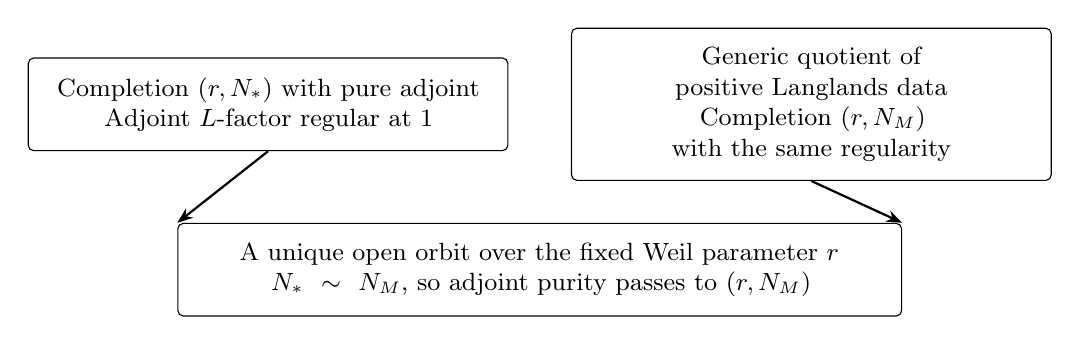
\begin{tikzpicture}[
 box/.style={draw,rounded corners=2pt,align=center,text width=5.6cm,
             inner sep=7pt,font=\small},
 arr/.style={-{Stealth[length=2mm]},thick}]
 \node[box] (global) at (0,0)
  {Completion $(r,N_*)$ with pure adjoint\\
   Adjoint $L$-factor regular at $1$};
 \node[box] (local) at (6.9,0)
  {Generic quotient of\\positive Langlands data\\
   Completion $(r,N_M)$ with the same regularity};
 \node[box,text width=8.7cm] (orbit) at (3.45,-2.1)
  {A unique open orbit over the fixed Weil parameter $r$\\
   $N_*\sim N_M$, so adjoint purity passes to $(r,N_M)$};
 \draw[arr] (global.south) -- (orbit.north west);
 \draw[arr] (local.south) -- (orbit.north east);
\end{tikzpicture}
\caption{The local comparison uses two independently obtained
monodromy operators. Adjoint regularity identifies their orbits
over the fixed Weil parameter $r$.}
\label{fig:comparison}
\end{figure}

Purity now passes to the positive dual nilradical, a direct summand
of the adjoint Weil--Deligne representation. A pure weight-zero
representation has Frobenius determinant of absolute value $1$.
The positive exponent $\nu$ makes that same determinant strictly
smaller than $1$. This contradiction proves the local criterion.

Globally, the companion theorem makes every unramified component
tempered. The adjoint local system attached to an occurring
excursion parameter is consequently pointwise pure of weight zero.
Deligne's theorem on local monodromy for curves
\cite[Th\'eor\`eme~1.8.4]{DeligneWeilII} supplies a pure adjoint
completion at each place. Semisimple local-global compatibility
identifies its Weil part with the parameter of $\pi_v$, and the
local criterion applies.

Section~\ref{sec:parameters} fixes conventions and states the
parameter inputs. Section~\ref{sec:monodromy} proves the monodromy
and purity lemmas. Section~\ref{sec:coefficients} establishes the
local-coefficient comparison, including its behavior under
specialization. Section~\ref{sec:local-criterion} proves the local
criterion, and Section~\ref{sec:global} applies it to the global
representation.

\section{Local conventions and parameter theorems}\label{sec:parameters}

We record the precise parameter theorems used below and explain how their
semisimple Weil parameters relate to monodromy. The distinction is essential:
the global theorem and the tempered-completion theorem will produce two
potentially different monodromy operators over the same Weil parameter.

\subsection{Groups, induction, and Whittaker characters}

Let $k$ be a nonarchimedean local field of positive characteristic, with
residue field of cardinality $Q$. Fix a split adjoint absolutely simple
group $G$ over $k$, a split maximal torus $T$, and a Borel subgroup $B=TU$.
In the local arguments, $H$ denotes either $G$ or a standard Levi subgroup
of $G$; a standard parabolic of $H$ is written $P=MR$. Dual groups have
compatible positive systems, so positive coroots of $H$ are positive roots
of $\widehat H$. Put $\widehat{\mathfrak n}=\Lie(\widehat R)$.
All parabolic induction is normalized and is denoted $I_P^H$.

For a split group, a Whittaker character is a smooth unitary character of
its maximal unipotent subgroup that is nontrivial on every simple root
group. A smooth representation is \emph{generic} if it admits a nonzero
equivariant functional for such a character. We use uniqueness of Whittaker
functionals for irreducible generic representations, heredity under
normalized induction, and exactness of twisted unipotent coinvariants.
These statements, and the local-coefficient constructions based on them,
are valid over local function fields; see \cite[Sections~1--2]{LomeliLS}
and \cite[Section~2]{DCHL}. Exactness is also
\cite[Proposition~1.9(a)]{BernsteinZelevinsky}. For the foundational uniqueness and heredity
results, see also \cite[Th\'eor\`emes~2 and~4]{Rodier}.

The following elementary observation ensures that Whittaker data can be
chosen compatibly throughout the argument, even in small characteristic.

\begin{lemma}\label{lem:whittaker}
Every standard Levi subgroup $H$ of $G$ has split connected center.
Every smooth character of its maximal unipotent subgroup is trivial on
the nonsimple positive root groups. Its nondegenerate unitary characters
form a single $T(k)$-orbit.
\end{lemma}

\begin{proof}
Because $G$ is adjoint, its simple roots are a $\mathbb Z$-basis of
$X^*(T)$. The center of $H$ is the simultaneous kernel of a subset of
these coordinate characters, hence is a split torus. The same basis
allows arbitrary independent rescaling of the simple-root coordinates
belonging to $H$. Once triviality on nonsimple root groups is known,
additive self-duality of $k$ proves the orbit assertion.

To prove that triviality, a nonsimple positive root may be written as a
sum of two positive roots. The full root subsystem in their span reduces
the question to $A_2$, $B_2$, or $G_2$, with its induced positive system.
In $A_2$ the usual commutator is a parametrization of the nonsimple root
group. For $B_2$ or $G_2$, write $a,b$ for the short and long simple roots.
In $G_2$ first kill the highest root group $U_{3a+2b}$ using
$[U_b,U_{3a+b}]$, whose coefficient is $\pm1$. Modulo that group, the
commutator $[x_a(u),x_b(t)]$ has factors
\[
 x_{ja+b}(\epsilon_j u^j t),\qquad \epsilon_j\in\{1,-1\},
\]
with $1\leq j\leq2$ in $B_2$ and $1\leq j\leq3$ in $G_2$.
Fix a nontrivial additive character $\psi$ of $k$, and write the
restriction of the given character to $U_{ja+b}$ as
$x_{ja+b}(t)\mapsto\psi(c_jt)$. It kills commutators, so
\[
 \psi\left(t\sum_j\epsilon_jc_ju^j\right)=1
 \quad\text{for every }u,t\in k.
\]
Varying $t$ gives $\sum_j\epsilon_jc_ju^j=0$ for every $u$.
Since $k$ is infinite, all $c_j$ vanish. This polynomial argument uses no
division by $2$ or $3$ and remains valid in those characteristics.
\end{proof}

Write $\mathfrak a_{M,\C}^*=X^*(M)\otimes_{\mathbb Z}\C$.
For $z\in\mathfrak a_{M,\C}^*$, the notation $\sigma_z$ denotes the
unramified twist in which $s\chi$ acts as $|\chi|^s$.
Via duality, $X^*(M)$ is the cocharacter lattice of
$Z(\widehat M)^\circ$; a central weight $b$ on a representation of
$\widehat M$ therefore pairs with $z$, giving $b(z)$.
In particular, the weights on $\widehat{\mathfrak n}$ satisfy
$b(\nu)>0$ when $\nu$ is in the open positive chamber for $P$.

\subsection{Weil--Deligne parameters and local factors}

Fix $\ell\ne\operatorname{char}(k)$ and an isomorphism
$\iota:\overline{\Q}_\ell\simeq\C$. All absolute values of coefficients
below are taken after $\iota$. Choose the square roots in normalized
induction and in the parameter theorems to correspond to positive real
square roots. We use geometric Frobenius $\Fr$, so $|\Fr|=Q^{-1}$.
Local class field theory sends a uniformizer to geometric Frobenius,
and Satake parameters are normalized accordingly. Thus a twist by
$|\chi|^s$ on representations gives the same $|\cdot|^s$-twist on
parameters.

A Frobenius-semisimple Weil--Deligne parameter for $H$ is a pair $(r,N)$,
where $r:W_k\longrightarrow\widehat H(\C)$ has finite inertia image and
semisimple Frobenius, and $N\in\Lie(\widehat H)$ is nilpotent with
\begin{equation}\label{eq:wd-relation}
 \Ad(r(w))N=|w|N.
\end{equation}
For an algebraic representation of $\widehat H$ on $V$, use the same
symbols for the induced operators and set
\begin{equation}\label{eq:local-factor}
 L(s,V)=\det\left(1-Q^{-s}r(\Fr)\mid(\ker N)^{r(I_k)}\right)^{-1}.
\end{equation}
This is a reciprocal polynomial in $Q^{-s}$, with constant term $1$;
in particular, it has no zeros. We often write $L(s,a\circ(r,N))$ when
the algebraic representation $a$ needs to be specified.

A tempered $L$-parameter is a homomorphism
$\phi:W_k\times\SL_2(\C)\longrightarrow\widehat H(\C)$, algebraic on
$\SL_2$, whose Weil image is bounded. Its associated pair is
\begin{equation}\label{eq:completion}
 r(w)=\phi\left(w,
       \begin{pmatrix}|w|^{1/2}&0\\0&|w|^{-1/2}\end{pmatrix}\right),
 \qquad
 N=d\phi\begin{pmatrix}0&1\\0&0\end{pmatrix}.
\end{equation}
Thus the Weil part $r$ of a tempered completion need not itself be
bounded. This familiar distinction is the reason to retain monodromy.

We write $f\doteq g$ for equality up to a nonzero constant times a
monomial in the exponential unramified-twist coordinates. Finite covers
of twist tori are allowed. In additive coordinates, the omitted factor
is a constant times the exponential of a linear form, hence is
holomorphic and nowhere zero. In one variable it has the form $cQ^{-as}$.

\subsection{The parameter inputs}

We use the following forms of the global and local parameter theorems.
They specify the precise information carried from representations to
parameters; no compatibility of monodromy is included.

\begin{theorem}[Lafforgue; Genestier--Lafforgue]\label{thm:parameters}
For the split groups considered here the following hold.
\begin{enumerate}[label=\textup{(\roman*)}]
\item An irreducible smooth local representation $\sigma$ has a
semisimple Weil parameter $\rho_\sigma$, with finite inertia image.
The parametrization is compatible with normalized parabolic induction,
tori and local class field theory, group isomorphisms, central characters,
and twists through algebraic characters of the group.
\item A cuspidal automorphic representation $\Pi$ over a function field,
with finite-order central character, occurs in an excursion summand
with a semisimple global parameter $\Sigma_\Pi$. This parameter is
defined over a finite extension of $\Q_\ell$ and matches normalized
Satake parameters away from a finite set.
\item At every place $v$, the semisimplification of
$\Sigma_\Pi|_{W_{F_v}}$ is conjugate to $\rho_{\Pi_v}$.
\end{enumerate}
\end{theorem}

The global statement is \cite[Th\'eor\`eme~0.1]{VLafforgue}; the local
statements, including representations without an integrality condition,
are \cite[Th\'eor\`eme~0.1 and Remarque~0.2]{GenestierLafforgue}.
For compatibility with central characters, apply the functoriality for
homomorphisms with normal image to the inclusion of the central split
torus.

Here is how to interpret the coefficient and occurrence assertions for
complex representations. A finite-order central character allows a
cocompact central lattice in its kernel. Fixed-level cusp spaces modulo
that lattice are finite-dimensional and commute with coefficient
extension. Project an irreducible Hecke module of level invariants to
any excursion summand where its projection is nonzero; that projection
is injective, so it supplies the required occurrence. Uniqueness of the
excursion parameter of $\Pi$ is unnecessary. For the adjoint group no
central lattice is needed.

Locally, after transport by $\iota$, irreducibles may be realized over a
finite extension of $\Q_\ell$. Indeed a fixed-compact-open Hecke algebra
over $\Q_\ell$ is of finite type
\cite[Theorem~1.1]{DHKMFiniteness2024}, so its finite-dimensional simple
module over $\overline{\Q}_\ell$ descends to
such an extension. The corresponding irreducible representation also
descends: form induction from this Hecke module and quotient by the
largest subrepresentation with zero invariants under that compact
open subgroup. The latter subrepresentation is characterized by
vanishing of every averaged translate, a condition compatible with
scalar extension. This permits use of the finite-extension formulations
of the parameter theorems.

\begin{theorem}[Gan--Harris--Sawin, with Beuzart-Plessis]
\label{thm:tempered-completion}
If $\sigma$ is tempered on a standard Levi subgroup $M$ of $G$, then
$\rho_\sigma$ has a tempered completion $(\rho_\sigma,N_M)$ as in
\eqref{eq:completion}. This holds in every positive characteristic.
\end{theorem}

\begin{proof}[Explanation of the cited form]
The published \cite[Theorem~1.2 and Corollary~1.3]{GHS} give an
\emph{essentially} tempered completion for arbitrary connected reductive
groups over local function fields. Thus its Weil image is bounded modulo
the center. Since $\sigma$ is tempered, its central character is unitary.
By Theorem~\ref{thm:parameters}, the dual morphism
$\widehat M\to\widehat{Z(M)}$ has bounded image on the parameter.
Root data show that its characters span the rational character space
of the abelian quotient of $\widehat M$. Moreover, the $\SL_2$ factor
dies in that quotient. Hence the Weil image of the completion is
bounded in the abelian quotient as well. The map from $\widehat M$ to
the product of its adjoint and abelian quotients has finite kernel;
boundedness in these two quotients therefore gives boundedness in
$\widehat M$ itself.
\end{proof}

\subsection{The Weil part of a global restriction}

The local monodromy theorem turns a restriction of $\Sigma_\Pi$ into a
Weil--Deligne pair. The next observation verifies that its
Frobenius-semisimple Weil part is exactly the parameter in
Theorem~\ref{thm:parameters}(iii), also as a dual-group-valued parameter.

\begin{lemma}\label{lem:wd-semisimplification}
Let $\Sigma$ be a continuous $\ell$-adic representation of a local
decomposition group into $\widehat H$, defined over a finite extension
of $\Q_\ell$. If $(r,N)$ is its Frobenius-semisimplified Weil--Deligne
pair, then $r$ is conjugate to the semisimplification of $\Sigma|_{W_k}$.
\end{lemma}

\begin{proof}
Before Frobenius semisimplification, write the pair as $(r_0,N)$, with
$r_0(I_k)$ finite. The construction takes place in $\widehat H$:
in a faithful linear representation the unipotent logarithm lies in
its Lie algebra, and $\Sigma$ on the Weil group is obtained from $r_0$
by multiplying by the appropriate exponentials of $N$.

Write $r_0(\Fr)=hu$ for its commuting semisimple and unipotent parts.
Some positive power of $r_0(\Fr)$ centralizes the finite inertia image.
Jordan decomposition in that centralizer shows that a power of $u$,
and hence $u$, centralizes it. The relation
$\Ad(hu)N=Q^{-1}N$ gives $\Ad(h)N=Q^{-1}N$ and $\Ad(u)N=N$.
Replacing $hu$ by $h$ thus defines a Weil parameter $r$ with the same
finite inertia. The identity component of the Zariski closure of $r(W_k)$
is toral, so $r$ is semisimple.

Let $S$ be the identity component of the Zariski closure of the cyclic
group generated by $h$. It is a torus centralizing $r_0(I_k)$ and $u$.
If $N\ne0$, its weight on the line $\C N$ is nontrivial, because
$Q^{-1}$ is not a root of unity. A cocharacter of $S$ can therefore
contract $N$ to zero while fixing $r_0$. This realizes removal of the
monodromy exponentials as a conjugation limit in $\widehat H$.
Next, the centralizer of $r$ has reductive identity component and contains
the unipotent element $u$. A cocharacter in that centralizer contracts
$u$ to the identity. These two limits preserve semisimplification and
leave precisely $r$. Finally, density of the Weil group in the
decomposition group gives the same Zariski closure for both images.
\end{proof}

Thus a global restriction and a tempered local completion can have the
same $r$ while retaining distinct operators $N$. The next section gives
two ways to work with this distinction: an $L$-factor ratio that forgets
$N$, and a regularity condition that determines $N$ up to conjugacy.

\section{Adjoint regularity and monodromy}
\label{sec:monodromy}

The semisimple Weil parameter does not determine individual local
$L$-factors, since those factors also involve monodromy.  We first show
that the ratio occurring in a local functional equation is nevertheless
determined up to a unit.  We then explain how purity controls local
$L$-factors and determinants.  Finally, we prove that regularity of the
adjoint $L$-factor at $1$ determines the monodromy orbit.  These statements
will allow us to compare two monodromy operators once their semisimple
Weil parameters have been identified, without assuming compatibility of
the monodromy operators themselves.

\subsection{A ratio independent of monodromy}

\begin{lemma}\label{lem:monodromy-ratio}
Let $r$ be a Frobenius-semisimple Weil representation on a
finite-dimensional complex vector space $V$, with finite inertial
image.  If $N$ and $N'$ are nilpotent operators such that $(r,N)$ and
$(r,N')$ are Weil--Deligne representations, then
\[
 \frac{L(1-s,(r,N)^\vee)}{L(s,(r,N))}
 \doteq
 \frac{L(1-s,(r,N')^\vee)}{L(s,(r,N'))}.
\]
More precisely, put $W=V^{r(I_k)}$, $K=\ker(N|_W)$, and
$F=r(\mathrm{Fr})$.  If $R_N(s)$ denotes the ratio on the left, then
\begin{equation}\label{eq:monodromy-ratio-unit}
 \frac{R_0(s)}{R_N(s)}
   =\det\bigl(-Q^{-s}F\mid W/K\bigr).
\end{equation}
\end{lemma}

\begin{proof}
The operator $N$ commutes with inertia and satisfies
$FN=Q^{-1}NF$.  Thus $N$ identifies $W/K$ with $NW$, multiplying
Frobenius eigenvalues by $Q^{-1}$.  Averaging over the finite inertia
image identifies $(V^\vee)^{r^\vee(I_k)}$ with $W^\vee$.
The dual monodromy operator is $-N^{\mathsf t}$.  On $W^\vee$ its
kernel is the annihilator of $NW$, so restriction of functionals gives
the Frobenius-equivariant isomorphism
\[
 W^\vee/\ker(-N^{\mathsf t})\simeq (NW)^\vee.
\]
Consequently, if $c$ is a Frobenius eigenvalue on $W/K$, the
corresponding eigenvalue on this dual quotient is $Qc^{-1}$.
Writing $x=Q^{-s}$ and comparing the determinants for $N$ and $0$
gives
\[
 \frac{R_0(s)}{R_N(s)}
   =\prod_c\frac{1-xc}{1-Q^{-1}x^{-1}(Qc^{-1})}
   =\prod_c(-xc),
\]
where the eigenvalues are counted with multiplicity.  This proves
\eqref{eq:monodromy-ratio-unit}, as an identity of rational functions
in $x$.  Its right-hand side is a nonzero constant times a monomial,
and comparison through $N=0$ proves the assertion for $N$ and $N'$.
\end{proof}

\subsection{Consequences of purity}

Recall that the \emph{monodromy filtration centered at zero} of a
nilpotent operator $N$ on $V$ is the unique finite increasing
filtration $M_\bullet V$, indexed by the integers, satisfying
\[
 N(M_jV)\subset M_{j-2}V,
 \qquad
 N^j:\operatorname{Gr}^{M}_jV
      \xrightarrow{\ \sim\ }
      \operatorname{Gr}^{M}_{-j}V
 \quad (j\geq 0).
\]
Here $M_jV=0$ for sufficiently negative $j$ and $M_jV=V$ for
sufficiently positive $j$.  On a Jordan chain
$v,Nv,\ldots,N^dv$, the successive vectors have degrees
$d,d-2,\ldots,-d$.  This description constructs the filtration and
shows that it commutes with direct sums.  Its uniqueness also shows
that the Weil action preserves it, since conjugation by $r(w)$
multiplies $N$ by the nonzero scalar $|w|$.

We say that $(r,N)$ is \emph{pure of weight zero}, with respect to the
fixed complex realization of the coefficients, if every Frobenius
eigenvalue on $\operatorname{Gr}^{M}_jV$ has absolute value
$Q^{j/2}$.  When $N=0$, this says that all eigenvalues of
$r(\mathrm{Fr})$ have absolute value $1$.  Nonzero monodromy allows
eigenvalues of different absolute values, arranged in symmetric
Jordan chains.

\begin{lemma}\label{lem:pure-determinant}
Let $(r,N)$ be a finite-dimensional Frobenius-semisimple
Weil--Deligne representation, pure of weight zero.  Then
$L(s,(r,N))$ is holomorphic and nonzero for $\operatorname{Re}(s)>0$,
and
\begin{equation}\label{eq:pure-determinant}
 \left|\det r(\mathrm{Fr})\right|=1.
\end{equation}
Every Weil--Deligne direct summand of $(r,N)$ is also pure of weight
zero and satisfies these conclusions.
\end{lemma}

\begin{proof}
The bottom vector of a Jordan chain of length $d+1$ has monodromy
degree $-d$.  Hence $\ker N\subset M_0V$.  Purity implies that all
Frobenius eigenvalues on $M_0V$, and therefore on $(\ker N)^{I_k}$,
have absolute value at most $1$.  If $\operatorname{Re}(s)>0$, each
factor $1-Q^{-s}c$ in the defining determinant of the local
$L$-factor is nonzero.  The asserted holomorphy and nonvanishing
follow.

The defining isomorphisms of the monodromy filtration give
$\dim\operatorname{Gr}^{M}_jV
 =\dim\operatorname{Gr}^{M}_{-j}V$.  Taking the determinant on the
graded spaces therefore gives
\[
 \left|\det r(\mathrm{Fr})\right|
   =Q^{\frac12\sum_j j\dim\operatorname{Gr}^{M}_jV}=1.
\]
Finally, the monodromy filtration of a direct sum is the direct sum
of its monodromy filtrations.  Each graded space of a
Weil--Deligne summand is consequently a Frobenius-stable direct
summand of the corresponding graded space of $V$, and inherits its
purity.
\end{proof}

For example, take trivial inertia on $V=\mathbb C e_1\oplus
\mathbb C e_2$ and set
\[
 r(\mathrm{Fr})=
 \begin{pmatrix}Q^{-1/2}&0\\0&Q^{1/2}\end{pmatrix},
 \qquad
 Ne_2=e_1,\quad Ne_1=0.
\]
The degrees of $e_1,e_2$ are $-1,1$, so this representation is pure
of weight zero although the image of $r$ is unbounded.  It comes
from the $L$-parameter trivial on $W_k$ and standard on
$\mathrm{SL}_2(\mathbb C)$.  Replacing $N$ by $0$ destroys purity
and introduces a pole at $s=1/2$ in the local $L$-factor.  This is
why boundedness of the Weil part and purity of a completed
Weil--Deligne representation must be distinguished.

\subsection{Adjoint regularity determines the orbit}

The next proposition is the implication from adjoint regularity to an
open monodromy orbit established in
\cite[Proposition~3.5]{CDFZ2025} and
\cite[Proposition~6.10]{DHKM2026}.  We give the elementary argument in
the semisimple case needed here.  The Killing form identifies the
obstruction to an orbit being open with the space responsible for a
pole of the adjoint $L$-factor at~$1$.

\begin{proposition}\label{prop:open-orbit}
Let $\widehat G$ be a connected semisimple complex algebraic group,
and let $r:W_k\to\widehat G$ be a Frobenius-semisimple Weil
parameter with finite inertial image.  Write
\[
 \mathfrak e=\operatorname{Lie}(\widehat G)^{r(I_k)},
 \qquad
 \mathfrak e_a=
 \ker\bigl(\operatorname{Ad}(r(\mathrm{Fr}))-a
                 \mid\mathfrak e\bigr)
 \quad(a\in\mathbb C^\times),
\]
and let $C=Z_{\widehat G}(r(W_k))$.  If $(r,N)$ is a
Weil--Deligne parameter and $L(s,\operatorname{Ad}\circ(r,N))$
is regular at $s=1$, then the orbit $C\cdot N$ is open in
$\mathfrak e_{Q^{-1}}$.
In particular, if $N_1,N_2$ are two monodromy operators over $r$
whose adjoint $L$-factors are regular at $1$, then some $c\in C$
satisfies $\operatorname{Ad}(c)N_1=N_2$.
\end{proposition}

\begin{proof}
The Weil--Deligne relation places $N$ in
$\mathfrak e_{Q^{-1}}$.  On the adjoint representation its
monodromy is $\operatorname{ad}(N)$, so regularity at $1$ is
equivalent to
\begin{equation}\label{eq:adjoint-pole-kernel}
 \ker(\operatorname{ad}N)\cap\mathfrak e_Q=0.
\end{equation}
Indeed, a pole at $1$ means that Frobenius has eigenvalue $Q$ on
$(\ker\operatorname{ad}N)^{r(I_k)}$.

Let $B$ be the Killing form of $\operatorname{Lie}(\widehat G)$.
Its restriction to $\mathfrak e$ is nondegenerate.  To see this,
average any vector over the finite inertia image: pairing it with
an inertia-invariant vector gives the same value before and after
averaging.  A vector orthogonal to $\mathfrak e$ inside
$\mathfrak e$ is therefore orthogonal to the entire Lie algebra,
and is zero.  Frobenius preserves $B$ and acts semisimply, so $B$
pairs $\mathfrak e_a$ perfectly with $\mathfrak e_{a^{-1}}$.

We have $\operatorname{Lie}(C)=\mathfrak e_1$.  The differential
of the orbit map at the identity is
\begin{equation}\label{eq:monodromy-orbit-tangent}
 \mathfrak e_1\longrightarrow\mathfrak e_{Q^{-1}},
 \qquad Y\longmapsto[Y,N].
\end{equation}
By invariance of $B$, its transpose under the preceding perfect
pairings is
\[
 \mathfrak e_Q\longrightarrow\mathfrak e_1,
 \qquad X\longmapsto[N,X].
\]
The kernel of this transpose is zero by
\eqref{eq:adjoint-pole-kernel}, so
\eqref{eq:monodromy-orbit-tangent} is surjective.  Algebraic group
orbits are smooth and locally closed in characteristic zero.
Thus $C\cdot N$ has the dimension of $\mathfrak e_{Q^{-1}}$ and
is open in that vector space.  Since the vector space is
irreducible, it has at most one open $C$-orbit.  This proves the
last assertion as well.
\end{proof}

\section{Local coefficients and semisimple parameters}
\label{sec:coefficients}

The comparison in this section expresses the divisor of a Shahidi local
coefficient in terms of the semisimple local parameter.  It applies to
arbitrary generic inducing representations, including ramified
supercuspidals.  We use multiplicativity to reduce to supercuspidal data,
and then isolate the prescribed place in a global functional equation.
Only the product of local factors occurring in a local coefficient is
needed.  Lemma~\ref{lem:monodromy-ratio} allows this product to be compared
without identifying monodromy operators.

Let $H$ be a split adjoint group under consideration, or a standard Levi
subgroup of such a group, over the local function field $k$.  Fix a split
maximal torus $T$, a Borel subgroup $B=TU$, and a nondegenerate character
$\psi$ of $U(k)$.  Write $P=MR$ for a proper standard parabolic subgroup
of $H$.  All induction is normalized, and we write
\[
 I_P^H(\sigma_z)=\operatorname{Ind}_{P(k)}^{H(k)}(\sigma_z).
\]
Here $\sigma$ is an irreducible generic representation of $M(k)$ and
$z\in\mathfrak a_{M,\mathbb C}^*=X^*(M)\otimes_{\mathbb Z}\mathbb C$.
Whittaker characters and Weyl representatives are chosen compatibly.
Lemma~\ref{lem:whittaker} gives a single torus orbit of nondegenerate
characters for these groups, so such a choice is possible for every
generic $\sigma$.

Let $w_H$ and $w_M$ denote the longest Weyl elements of $H$ and $M$, and
put $w=w_Hw_M$.  Let $P'$ be the standard parabolic with Levi
$wMw^{-1}$.  The standard intertwining operator
\[
 A_H(z,\sigma;w):I_P^H(\sigma_z)
       \longrightarrow I_{P'}^H((w\sigma)_{wz})
\]
is defined by its usual unipotent integral and meromorphic continuation.
In particular, $A_H$ has no normalization by local
$L$-functions.  We use the convention
\begin{equation}
 \lambda_{\mathrm{source}}(z)
   =C_H(z,\sigma)\,\lambda_{\mathrm{target}}(wz)
                         \circ A_H(z,\sigma;w)
 \label{eq:coefficient-definition}
\end{equation}
for the local coefficient.  We also use this definition for a Weyl
element carrying the simple roots of its source Levi into the ambient
simple roots.  These are the intertwiners that occur in multiplicativity.

Let $\widehat P=\widehat M\widehat R$ be the corresponding standard
parabolic in $\widehat H$.  Decompose its unipotent Lie algebra under the
connected center of $\widehat M$:
\begin{equation}
 \widehat{\mathfrak n}
       :=\operatorname{Lie}(\widehat R)=\bigoplus_b V_b.
 \label{eq:central-weight-decomposition}
\end{equation}
The index $b$ runs over the weights that occur, $r_b$ is the representation
of $\widehat M$ on $V_b$, and $b(z)$ is the pairing with the central
cocharacter specified by the twist $z$.

\begin{proposition}[Comparison of local coefficients]
\label{prop:comparison}
For $H,P,M$, and $\sigma$ as above, let
$(\rho_\sigma,N_\sigma)$ be any Weil--Deligne pair in $\widehat M$ with
Weil part the semisimple local parameter of $\sigma$.  Then
\begin{equation}
 C_H(z,\sigma)\ \doteq\
 \prod_b
 \frac{L\bigl(1-b(z),r_b^\vee\circ(\rho_\sigma,N_\sigma)\bigr)}
      {L\bigl(b(z),r_b\circ(\rho_\sigma,N_\sigma)\bigr)}.
 \label{eq:coefficient-comparison}
\end{equation}
In particular, one may take $N_\sigma=0$.  The equality is an identity of
meromorphic functions of the unramified twists, up to a nonzero constant
times a monomial in twist coordinates.
\end{proposition}

We first explain how local coefficients behave under specialization and
induction in stages.  We then prove the rank-one and principal-series
cases of the proposition.  Globalization supplies the remaining
supercuspidal case.  The local-coefficient constructions and the crude
functional equation are those of Lomel\'i
\cite[\S\S1--2 and Theorem~4.3]{LomeliLS}; the globalization method is
that of Gan--Lomel\'i \cite[Theorem~1.1 and \S5]{GanLomeli}.
For the related construction of $\gamma$-factors from semisimple
parameters, see also \cite[Section~7]{GenestierLafforgue}.

\subsection{Whittaker lines in families}

For a smooth representation $V$ of $H(k)$, write $V_{U,\psi}$ for its
twisted coinvariants.  When $V=I_P^H(\sigma_z)$ with $\sigma$ generic,
these coinvariants are one-dimensional.  The scalar of the standard
intertwining operator on this line is the inverse local coefficient.
To use this description at a reducibility point, one must choose
generators that remain nonzero after specialization.

Choose a finite cover of the torus of unramified twists on which the
characters in use are algebraic, and let $\mathcal A$ be its Laurent
polynomial coordinate ring.  The family $\sigma_z$ is a smooth
$\mathcal A[M(k)]$-module, and its induced family is a smooth
$\mathcal A[H(k)]$-module.  Meromorphic operators are obtained by
extending scalars to the fraction field of $\mathcal A$.

\begin{lemma}[Whittaker lines and specialization]
\label{lem:whittaker-family}
The twisted coinvariants of the induced family $I_P^H(\sigma_z)$ form a
free rank-one $\mathcal A$-module, and this description commutes with
specialization of $z$.  The Jacquet-integral Whittaker functionals give a
generator of its dual whose specialization is nonzero at every twist.
Consequently, the inverse scalar induced by $A_H$ on these lines is
$C_H(z,\sigma)$ up to a unit of $\mathcal A$.
\end{lemma}

\begin{proof}
The twisted Jacquet functor is exact over $\mathcal A$.  Indeed, the
unipotent group $U(k)$ is an increasing union of compact open subgroups.
On each such subgroup, twisted averaging is an idempotent, since
$\mathcal A$ is a complex algebra.  Taking the resulting filtered
colimit proves exactness.  The same description shows that twisted
coinvariants commute with scalar extension, including specialization.

Apply this functor to the Bruhat filtration of parabolic induction.
For a representative $x$ of $W_M\backslash W_H$, the corresponding
subquotient consists of sections with compact support modulo $P(k)$
on the cell $P(k)\dot xU(k)$.  As a $U(k)$-representation, it is compact
induction from
\[
 U(k)\cap\dot x^{-1}P(k)\dot x,
\]
with the fiber action obtained from the inducing representation.
Its twisted coinvariants are therefore computed on the fiber.  All
unramified twists and modulus characters are trivial on the unipotent
groups in this calculation, so the calculation is unchanged over
$\mathcal A$.

Every cell other than the open one has a simple root subgroup of $U$
whose conjugate lies in $R$.  It acts trivially on the fiber and
nontrivially through $\psi$, so that cell contributes no twisted
coinvariants.  For completeness, take $x$ minimal on the left modulo
$W_M$.  If no simple root is sent to a positive root outside $M$, every
$x\alpha$ for $\alpha$ simple is either negative or a positive Levi
root. Thus the coefficients outside the Levi simple system of every
$x\beta$, $\beta$ positive, are nonpositive. In particular, $x\beta$
cannot be a positive root outside $M$. It follows that $x^{-1}$ sends
all positive roots outside $M$ to negative roots, which characterizes
the representative of the open cell.

On the open cell, the remaining coinvariant calculation is precisely
the Whittaker coinvariant space of $\sigma$, with the character
transported by the chosen representative.  This space is
one-dimensional by Whittaker uniqueness.  Hence the induced family's
coinvariants are its tensor product with $\mathcal A$, as asserted.
This is the usual open-cell proof of Whittaker heredity, now carried
out over the coefficient ring.

The open-cell submodule therefore induces an isomorphism on twisted
coinvariants.  Its unipotent integral, applied to a fixed Whittaker
functional of $\sigma$, extends uniquely through this isomorphism to
an $\mathcal A$-linear Whittaker functional on the entire induced
family.  In a convergence chamber this functional and the usual
Jacquet integral agree on the open-cell submodule, and hence agree
everywhere.  Meromorphic continuation consequently identifies the
Jacquet functional with this algebraic functional.  In particular,
its evaluations on algebraic sections are Laurent polynomials, as
also recalled in \cite[\S1.2]{LomeliLS}.

To see that specialization is nonzero, choose a vector on which the
fixed Whittaker functional of $\sigma$ is $1$ and a compactly supported
function in the open-cell unipotent coordinates whose $\psi$-weighted
integral is $1$.  The resulting algebraic section has Whittaker value
$1$ at every twist.  Thus the regular functional just constructed
never specializes to zero and generates the dual coinvariant line.

Equation~\eqref{eq:coefficient-definition} now identifies the local
coefficient with the inverse scalar on these free lines.  Two
generators of a free rank-one Laurent polynomial module differ by a
unit, hence by a nonzero constant times a monomial.  Haar measures and
compatible Weyl representatives change the formula only by such
units.  Torus conjugation of the Whittaker character also identifies
these lines over $\mathcal A$ and commutes with the intertwining
calculation, with the same consequence.
\end{proof}

\subsection{Elementary intertwiners and reduction of the inducing data}

We record the root decomposition that governs both sides of
\eqref{eq:coefficient-comparison}.  For a Weyl element $v$, set
\[
 \operatorname{Inv}(v)
   =\{\beta\in\Phi_H^+:v\beta\in-\Phi_H^+\}.
\]
For a standard Levi $L$, write $\Delta_L$ for its simple roots.

\begin{lemma}[Elementary factorization]
\label{lem:elementary-moves}
Let $L$ be a standard Levi of $H$, and suppose $v\Delta_L\subseteq
\Delta_H$.  There is a length-additive factorization
\[
 v=v_t\cdots v_1
\]
with the following properties.  Put $v_{<j}=v_{j-1}\cdots v_1$ and
$L_j=v_{<j}Lv_{<j}^{-1}$.  Then $L_j$ is standard, it is a maximal
proper Levi in a standard Levi subgroup $H_j$, and
\[
 \Delta_{H_j}=\Delta_{L_j}\cup\{\alpha_j\},\qquad
 v_j=w_{H_j}w_{L_j}.
\]
Moreover,
\begin{equation}
 \operatorname{Inv}(v)
   =\bigsqcup_{j=1}^t v_{<j}^{-1}\operatorname{Inv}(v_j).
 \label{eq:inversion-partition}
\end{equation}
The analogous partition holds for coroots.
\end{lemma}

\begin{proof}
If $v\ne1$, choose a simple root $\alpha$ with $v\alpha<0$.
Such a root is outside $\Delta_L$, since $v\Delta_L\subseteq\Delta_H$.
Let $H_1$ be the standard Levi obtained by adjoining $\alpha$ to
$\Delta_L$, and set $v_1=w_{H_1}w_L$.

Every positive root of $H_1$ outside $L$ has a strictly positive
$\alpha$-coefficient.  Its image under $v$ is a positive linear
combination of $v\alpha$ and roots in $v\Delta_L$.  The negative root
$v\alpha$ has a strictly negative coefficient outside $v\Delta_L$:
otherwise it would belong to the span of $v\Delta_L$, contradicting
$\alpha\notin\operatorname{span}(\Delta_L)$.  This coefficient cannot
be canceled by the other summands.  The image root is therefore
negative.  It follows that
\[
 \operatorname{Inv}(v_1)
   =\Phi_{H_1}^+\setminus\Phi_L^+
   \subseteq\operatorname{Inv}(v).
\]
Consequently $v_1$ is a right factor with additive length.

The element $v_1$ carries $\Delta_L$ into the simple roots of $H_1$.
Replace $L$ by $v_1Lv_1^{-1}$ and $v$ by $vv_1^{-1}$, which still
carries the new Levi simple system into $\Delta_H$.  The length has
strictly decreased, so iteration terminates.  The usual inversion-set
identity for a product with additive lengths gives
\eqref{eq:inversion-partition}.  Applying the same argument to the dual
root system gives its coroot version.
\end{proof}

The standard intertwining integrals factor according to
Lemma~\ref{lem:elementary-moves}.  First one uses Fubini's theorem in
a convergence chamber, and then meromorphic continuation.  At each
step, normalized induction in stages identifies the elementary
operator with the maximal-parabolic operator in $H_j$.  Taking
Whittaker scalars and using Lemma~\ref{lem:whittaker-family} therefore
gives multiplicativity of local coefficients, up to the allowed
units.  This is the multiplicativity of
\cite[Proposition~2.3]{LomeliLS}.

We explain more precisely how it reduces the inducing representation.
Suppose for the moment that $P$ is maximal in $H$, with omitted simple
root $\alpha$.  Let $\widetilde\alpha\in\mathfrak a_{M,\mathbb R}^*$
be proportional to the character giving the determinant on
$\operatorname{Lie}(R)$ and normalized by
\[
 \langle\widetilde\alpha,\alpha^\vee\rangle=1.
\]
Its pairing with every simple coroot of $M$ is zero.  The decomposition
\eqref{eq:central-weight-decomposition} is then conventionally written
\[
 \widehat{\mathfrak n}=\bigoplus_{i\geq1}V_i,\qquad
 V_i=\bigoplus_{\langle\widetilde\alpha,\beta^\vee\rangle=i}
                       \widehat{\mathfrak h}_{\beta^\vee},
\]
where $\widehat{\mathfrak h}_{\beta^\vee}$ is the corresponding root
space in $\operatorname{Lie}(\widehat H)$ and $i$ ranges over the
positive integers that occur.  Along
$z=s\widetilde\alpha$, the arguments in
\eqref{eq:coefficient-comparison} are $is$ and $1-is$.

Every other twist direction is a sum of this relative direction and a
direction in $X^*(H)\otimes\mathbb C$.  A twist from $H$ twists both
sides of the intertwiner and changes its Whittaker scalar by at most
a unit.  On the dual side it acts through $Z(\widehat H)^\circ$ and
acts trivially on $\widehat{\mathfrak n}$.  Thus it suffices to prove
the maximal-parabolic comparison on the relative line.

By the subrepresentation theorem, $\sigma$ embeds in normalized
induction in $M$ from a supercuspidal representation $\sigma_0$ of a
standard Levi $M_0\subseteq M$.  Exactness and heredity of Whittaker
coinvariants show that $\sigma_0$ is generic.  They also show that the
embedding induces an isomorphism on Whittaker lines, since both lines
are one-dimensional.  The same holds after every unramified twist.

The element $w=w_Hw_M$ carries the simple roots of $M_0$ into those of
$H$.  In the induced realization from $M_0$, its intertwining integral
still uses exactly the roots outside $M$ turned negative by $w$:
$w$ preserves the positive system of $M$ in its target Levi.  Thus
induction in stages identifies the intertwiner on $\sigma$ with the
restriction of this intertwiner on the smaller inducing data.  The
isomorphisms of Whittaker lines just established identify their local
coefficients, up to units.

Apply Lemma~\ref{lem:elementary-moves} with $L=M_0$, and write
$M_j=w_{<j}M_0w_{<j}^{-1}$ for the successive Levi subgroups.  At step $j$,
the inducing representation is the transport of $\sigma_0$ to $M_j$,
and the twist is $w_{<j}(s\widetilde\alpha)$.  Its relative coordinate
in $H_j$ is $c_js$, where
\begin{equation}
 c_j=\langle w_{<j}\widetilde\alpha,\alpha_j^\vee\rangle>0.
 \label{eq:relative-slope}
\end{equation}
Indeed, $w_{<j}^{-1}\alpha_j^\vee$ belongs to the original inversion
set of coroots, all of which are positive and outside $M$.  Pairing
with $\widetilde\alpha$ is strictly positive on this set.  Each
elementary coefficient consequently has a genuinely varying argument;
the reduction does not restrict a meromorphic coefficient to an
identically singular locus.

The same factorization decomposes the dual representations.  Transport
the nilradical Lie algebra for $M_j\subset H_j$ back by $w_{<j}^{-1}$.
It is invariant under $\widehat M_0$, because the original algebra is
invariant under $\widehat M_j$.  The coroot partition
\eqref{eq:inversion-partition} identifies their direct sum with
$\widehat{\mathfrak n}$ restricted to $\widehat M_0$.  A step summand
of relative degree $i_j$ has twist exponent $c_ji_js$.  To see this,
decompose $w_{<j}\widetilde\alpha$ into
$c_j\widetilde\alpha_j$ and a character direction from $H_j$; the
latter pairs to zero with every coroot in $H_j$.

Compatibility of semisimple parameters with normalized induction
identifies $\rho_\sigma$ with the parameter obtained from
$\rho_{\sigma_0}$.  Taking monodromy zero, the preceding decomposition
therefore makes the right side of
\eqref{eq:coefficient-comparison} the product of the right sides for
the elementary maximal parabolics.  We have proved that comparison
for maximal parabolics with supercuspidal inducing data implies
comparison for maximal parabolics with arbitrary generic data.

\subsection{The principal-series comparison}

The rank-one case supplies the local comparisons needed away from the
place prescribed in globalization.  If a maximal proper Levi $M$ is a
torus, the derived root system of $H$ has rank one.  The local
coefficient is the Tate gamma factor for the character obtained by
pulling $\sigma$ back along the coroot.  Tate's formula and local class
field theory give
\begin{equation}
 C_H(s\widetilde\alpha,\sigma)
   \ \doteq\
   \frac{L(1-s,r_1^\vee\circ\rho_\sigma)}
        {L(s,r_1\circ\rho_\sigma)}.
 \label{eq:rank-one-comparison}
\end{equation}
This calculation permits an arbitrary smooth inducing character;
see \cite[\S1.3]{LomeliLS}.  It also applies to the isogeny types
occurring here.  Pulling the integral back through the root
homomorphism from $\operatorname{SL}_2$ identifies the root groups
and the unipotent integration, and the inducing character pulls back
through the stated coroot.  Extra central tori have no effect on this
calculation.

An irreducible generic constituent of a principal series can be
embedded in a principal series, with a possibly Weyl-conjugate
inducing character, by the subrepresentation and supercuspidal
support theorems.  The preceding elementary factorization with
$M_0=T$ reduces its comparison to
\eqref{eq:rank-one-comparison}.  Thus the maximal-parabolic case of
\eqref{eq:coefficient-comparison} is already proved whenever the
inducing representation is a generic principal-series constituent.
In particular it is available for ramified principal series; an
Iwahori-fixed hypothesis is not needed.

\subsection{Globalization of supercuspidal data}

We now prove the remaining maximal-parabolic comparison.  Let
$\sigma$ be a generic supercuspidal representation of $M(k)$.  We
may first twist it so that its central character has finite order.
Indeed, $Z(M)$ is a split torus, a smooth character of its maximal
compact subgroup has finite image, and restriction
\[
 X^*(M)\longrightarrow X^*(Z(M))
\]
has finite cokernel.  Unramified twists can therefore adjust the
finitely many uniformizer values to roots of unity.  Twisting back
shifts the relative parameter $s$; the remaining twist direction is
from $H$ and has the behavior already described.  Twist compatibility
of semisimple parameters gives the identical shift on the proposed
Galois expression.

Write $k=k_0((t))$, and put $K=k_0(t)$.  Let $v_0$ be the rational
place $t=0$, so $K_{v_0}=k$.  Use the constant split models of $H$ and
$M$ over $K$.  The finite-order central character just obtained
extends to a finite-order automorphic character of $Z(M)(\mathbb A_K)$.
Here is an explicit extension, to check the central-character
hypothesis of globalization.

For one split central factor, the idele-class group of $K$ fits into
the split exact sequence
\begin{equation}
 1\longrightarrow
    \left(\prod_x\mathcal O_x^\times\right)/k_0^\times
   \longrightarrow K^\times\backslash\mathbb A_K^\times
   \xrightarrow{\deg}\mathbb Z\longrightarrow0.
 \label{eq:rational-idele-class-group}
\end{equation}
The degree-zero description follows from the triviality of
$\operatorname{Pic}^0(\mathbb P^1)$, and the uniformizer idele at
$v_0$ splits the degree map.  Prescribe the given unit character at
$v_0$, cancel its restriction to $k_0^\times$ using a character of
the residue field at infinity, and take trivial characters at the
remaining unit groups.  This defines a finite-order character of
the left group in \eqref{eq:rational-idele-class-group}.  Give the
degree generator the prescribed finite-order value of the local
character on $t$.  The resulting automorphic character has the
desired restriction at $v_0$.  Repeat for every split central factor.

Choose a nontrivial global additive character and the resulting
generic character of the Borel unipotent of $M$.  Its local character
at $v_0$ is in the torus orbit for which $\sigma$ is generic.  The
globalization theorem of Gan--Lomel\'i
\cite[Theorem~1.1]{GanLomeli} now produces a globally generic
cuspidal representation $\Pi$ of $M(\mathbb A_K)$ such that
\[
 \Pi_{v_0}\simeq\sigma,
 \qquad
 \Pi_x\text{ is a principal-series constituent for every }x\ne v_0,
\]
and whose central character is the finite-order character just
constructed.  Their theorem preserves the prescribed unipotent
period; for the Borel unipotent and a nondegenerate character this
is precisely global genericity.  It imposes no restriction on the
depth of $\sigma$ or on the positive characteristic.

Choose a global parameter $\Sigma$ occurring for $\Pi$, and enlarge
a finite set $S$ of places containing $v_0$ so that normalized
Satake matching and all unramified conditions for the crude
functional equation hold outside $S$.  For the maximal parabolic
under consideration, Lomel\'i's crude functional equation is
\begin{equation}
 \prod_i
 \frac{L^S(is,\Pi,r_i)}
      {L^S(1-is,\Pi,r_i^\vee)}
     \ \doteq\ \prod_{x\in S}
                 C_{H_x}(s\widetilde\alpha,\Pi_x).
 \label{eq:crude-functional-equation}
\end{equation}
In \cite[Theorem~4.3]{LomeliLS}, the denominator is written using
the contragredient $\widetilde\Pi$ and $r_i$.  At an unramified
place, contragredience inverts the Satake class up to the Levi Weyl
group, so those Euler factors are exactly the factors for $\Pi$
and $r_i^\vee$ displayed here.

The same partial Euler products are the partial $L$-functions of
$r_i\circ\Sigma$.  Write $\Phi_x$ for the local Weil--Deligne
parameter obtained from $\Sigma$ at $x$.  The functional equation
for a lisse sheaf on a curve, with ramified factors defined by
inertia invariants, gives
\begin{equation}
 \prod_i
 \frac{L^S(is,\Pi,r_i)}
      {L^S(1-is,\Pi,r_i^\vee)}
 \ \doteq\
 \prod_{x\in S}\prod_i
   \frac{L(1-is,r_i^\vee\circ\Phi_x)}
        {L(is,r_i\circ\Phi_x)}.
 \label{eq:galois-functional-equation}
\end{equation}
This is the usual curve functional equation
\cite[\S\S9--10]{DeligneConstants}; it follows from the trace formula
and duality for middle extensions, and does not require purity.
To check the direction of the local ratio, write the complete
functional equation as $L(s,V)=\varepsilon(s,V)L(1-s,V^\vee)$.
Removing the Euler factors in $S$ puts
$L_x(1-s,V^\vee)/L_x(s,V)$ on the right.  The global epsilon factor
is a nonzero constant times a monomial.  After the substitutions
$s\mapsto is$, its contribution has exactly the form suppressed
by $\doteq$.

The $\ell$-adic functional equation is an identity of rational
functions and is transported through the fixed coefficient
identification.  Its partial $L$-functions agree with the
automorphic ones because their Euler factors agree outside $S$.
The ramified factors are those of $\Phi_x$: the invariant stalk of
the lisse sheaf is the inertia-invariant kernel of its monodromy,
and Frobenius semisimplification does not change its determinant.

We can now isolate $v_0$.  For each $x\in S\setminus\{v_0\}$, the
representation $\Pi_x$ is generic and is a principal-series
constituent.  The principal-series comparison identifies its
factor in \eqref{eq:crude-functional-equation} with its factor in
\eqref{eq:galois-functional-equation}, up to a unit.  Local-global
compatibility, together with Lemma~\ref{lem:wd-semisimplification},
identifies the Weil part of the Frobenius-semisimplified pair $\Phi_x$
with $\rho_{\Pi_x}$.  Lemma~\ref{lem:monodromy-ratio} then permits
us to discard its monodromy in comparing the local ratios.
Cancellation leaves
\[
 C_H(s\widetilde\alpha,\sigma)
   \ \doteq\
   \prod_i
   \frac{L(1-is,r_i^\vee\circ\Phi_{v_0})}
        {L(is,r_i\circ\Phi_{v_0})}.
\]
At $v_0$ the same compatibility and
Lemma~\ref{lem:monodromy-ratio} replace $\Phi_{v_0}$ by
$(\rho_\sigma,0)$, or by any specified completion
$(\rho_\sigma,N_\sigma)$.  This proves
\eqref{eq:coefficient-comparison} for maximal parabolics with
supercuspidal data.  The reduction above proves it for every
generic inducing representation of a maximal Levi.

\subsection{Completion of the comparison for an arbitrary parabolic}

\begin{proof}[Proof of Proposition~\ref{prop:comparison}]
The maximal-parabolic case has just been proved.  For general $P=MR$,
apply Lemma~\ref{lem:elementary-moves} to $w=w_Hw_M$, now with
$L=M$, and put $M_j=w_{<j}Mw_{<j}^{-1}$.  At step $j$, the inducing data are transported from
$\sigma$ to $M_j$, and the twist is $w_{<j}z$.  Its relative
coordinate is
\[
 s_j(z)=\langle w_{<j}z,\alpha_j^\vee\rangle.
\]
This linear function is strictly positive on the positive chamber
for $P$, because its transported coroot lies outside $M$ in the
inversion partition.  In particular it is nonconstant.
The maximal-parabolic comparison is available for each step and
for every such twist, with directions from $H_j$ contributing
only units.  Multiplicativity gives the product of these step
formulas for $C_H(z,\sigma)$.

Use monodromy zero in these formulas.  Transporting the step
nilradicals back to $\widehat M$, the inversion partition gives
their direct sum as $\widehat{\mathfrak n}$.  On a step summand
of degree $i_j$, the twist exponent is $i_js_j(z)$, which is
exactly $b(z)$ for its connected-central weight in
\eqref{eq:central-weight-decomposition}.  Multiplicativity of
Artin $L$-factors for direct sums identifies the product of all
step expressions with the right side of
\eqref{eq:coefficient-comparison} for $N_\sigma=0$.
Finally Lemma~\ref{lem:monodromy-ratio}, applied to each $r_b$,
allows any Weil--Deligne completion with the same Weil part.
\end{proof}

\section{A local criterion for temperedness}\label{sec:local-criterion}

We now apply the local-coefficient comparison to a generic Langlands
quotient. It first supplies adjoint regularity for a completion built
from the tempered inducing representation. A completion of the same
semisimple parameter with pure adjoint will then force the inducing
exponent to vanish.

\begin{proposition}\label{prop:generic-regularity}
Let $G$ be split adjoint absolutely simple over $k$. Suppose a generic
irreducible representation $\tau$ is the Langlands quotient of
$I_P^G(\sigma_\nu)$, where $P=MR$ is a proper standard parabolic,
$\sigma$ is tempered, and $\nu$ is in the open positive chamber for $P$.
Choose a tempered completion $(\rho_\sigma,N_M)$ from
Theorem~\ref{thm:tempered-completion}, twist it by $\nu$, and include
it in $\widehat G$. The resulting pair $(r,N_M)$ has
$r\simeq\rho_\tau$ and
\[
 L(s,\Ad\circ(r,N_M))\quad\text{is regular at }s=1.
\]
\end{proposition}

\begin{proof}
Exactness and heredity of Whittaker coinvariants imply that $\sigma$
is generic. The assertion about $r$ follows from normalized-induction
and twist compatibility in Theorem~\ref{thm:parameters}.

Let $A(z)$ be the unnormalized long intertwiner on
$I_P^G(\sigma_z)$. For tempered inducing data, $A(z)$ is holomorphic
at $\nu$ and $\operatorname{im}A(\nu)$ is the Langlands quotient;
see \cite[Lemme~VII.4.1 and Th\'eor\`eme~VII.4.2]{Renard}
and \cite[Section~2.2]{DCHL}. Since this image is generic, exactness of
Whittaker coinvariants shows that the induced map on the two Whittaker
lines is nonzero at $\nu$. Using the algebraic trivializations with
nonvanishing specializations established in Section~\ref{sec:coefficients},
the local coefficient $C_G(z,\sigma)$, the inverse of that scalar,
is therefore holomorphic and nonzero at $\nu$.

Decompose $\widehat{\mathfrak n}=\bigoplus_bV_b$ under the connected
center of $\widehat M$, and denote its actions by $r_b$. For any
algebraic representation of a tempered parameter, the eigenvalues of
Frobenius on the kernel of monodromy have absolute value at most $1$.
Indeed, a highest weight $m\geq0$ of the $\SL_2$ factor contributes
$Q^{-m/2}$ in \eqref{eq:completion}, and the commuting Weil action
has eigenvalues of absolute value $1$. Consequently its local
$L$-factor is regular and nonzero when the argument has positive real part.

Since $b(\nu)>0$, every denominator in the identity of
Proposition~\ref{prop:comparison}, using $(\rho_\sigma,N_M)$, is
regular and nonzero at $z=\nu$. The product is also regular and
nonzero there. Local $L$-factors have no zeros, so none of the numerator
factors
\[
 L\bigl(1-b(\nu),r_b^\vee\circ(\rho_\sigma,N_M)\bigr)
\]
can have a pole.

Finally the decomposition into the Levi algebra and opposite nilradicals is
\[
 \Lie(\widehat G)=\Lie(\widehat M)
                   \oplus\widehat{\mathfrak n}
                   \oplus\widehat{\mathfrak n}^{-}.
\]
The Killing form identifies the last summand with the dual of the second.
On the first summand the central twist is trivial, so its factor is
regular at $1$ by temperedness. The second contributes arguments
$1+b(\nu)>0$. The third contributes the arguments $1-b(\nu)$ just
controlled by the numerator factors. Multiplication of these factors
proves the assertion.
\end{proof}

\begin{theorem}[Pure completion criterion]\label{thm:local-criterion}
Let $G$ be split adjoint absolutely simple over a local function field
$k$, and let $\tau$ be an irreducible generic smooth representation of
$G(k)$. Suppose $\rho_\tau$ admits a Weil--Deligne completion
$(\rho_\tau,N_*)$ whose adjoint representation is pure of weight zero.
Then $\tau$ is tempered.
\end{theorem}

\begin{proof}
Assume that $\tau$ is not tempered. By the Langlands classification it
has the description in Proposition~\ref{prop:generic-regularity}, with
$P$ proper and $\nu$ strictly positive. There is no real central twisting
direction for an adjoint group. Let $(r,N_M)$ be the completion in that
proposition, retaining its realization in the fixed dual Levi.
Transport the assumed completion by conjugacy to a pair $(r,N_*)$
over this same Weil parameter; its adjoint representation remains pure.

By Lemma~\ref{lem:pure-determinant}, the adjoint $L$-factor of
$(r,N_*)$ is regular at $1$, as is that of $(r,N_M)$ by
Proposition~\ref{prop:generic-regularity}.
Proposition~\ref{prop:open-orbit} therefore conjugates $N_M$ to $N_*$
by the centralizer of $r$. In particular,
$\Ad\circ(r,N_M)$ is pure of weight zero.

The Weil image lies in $\widehat M$, and $N_M$ lies in
$\Lie(\widehat M)$. Thus $\widehat{\mathfrak n}$ is a
Weil--Deligne direct summand of the adjoint representation.
Lemma~\ref{lem:pure-determinant} makes this summand pure of weight
zero and gives
\begin{equation}\label{eq:det-pure}
 \left|\det\bigl(r(\Fr)\mid\widehat{\mathfrak n}\bigr)\right|=1.
\end{equation}

We compute the same determinant before and after the twist. On every
central-weight summand $V_b$, the untwisted tempered parameter has
Weil determinant of absolute value $1$. Its $\SL_2$ factor has determinant
$1$, since $\SL_2$ has no nontrivial algebraic characters. Thus the
untwisted Weil--Deligne Frobenius determinant has absolute value $1$
on $V_b$. Twisting by $\nu$ multiplies each eigenvalue there by
$Q^{-b(\nu)}$. It follows that
\begin{equation}\label{eq:det-positive}
 \left|\det\bigl(r(\Fr)\mid\widehat{\mathfrak n}\bigr)\right|
   =Q^{-\sum_b b(\nu)\dim V_b}<1.
\end{equation}
The inequality is strict because $P$ is proper and every $b(\nu)>0$.
This contradicts \eqref{eq:det-pure}.
\end{proof}

The criterion separates the local issue from the global source of purity.
In particular it requires neither a full local Langlands correspondence
nor an identification of the two monodromy operators in advance.

\section{From unramified Ramanujan to every place}\label{sec:global}

We apply Theorem~\ref{thm:local-criterion} to a global parameter. The
only input specific to the global Ramanujan problem is the following
result from the companion manuscript \cite[Corollary~1.2]{UnramifiedRamanujan}.

\begin{theorem}[Unramified generalized Ramanujan]
\label{thm:unramified}
Let $F$ be the function field of a smooth projective geometrically
connected curve over a finite field. Let $G/F$ be split connected
adjoint absolutely simple. If a complex cuspidal automorphic
representation of $G(\A_F)$ has a generic unramified component, then
all its unramified components are tempered.
\end{theorem}

\begin{proof}[Proof of Theorem~\ref{thm:main}]
Write $F=\F_q(X)$ and choose a nonzero global Whittaker functional
for $\pi$. Every local component of its character is nondegenerate:
on a simple root group, an automorphic additive character is indexed
under adelic additive duality by a nonzero element of $F$, and is
therefore nontrivial at every place. Evaluating the global functional
on a pure tensor where it is nonzero, then varying the factor at $v$,
gives a nonzero local Whittaker functional on $\pi_v$. Thus every
$\pi_v$ is generic.

Almost every $\pi_v$ is unramified, so Theorem~\ref{thm:unramified}
applies. Choose an occurring global parameter $\Sigma$ as in
Theorem~\ref{thm:parameters}; $G$ has trivial center. On a sufficiently
small nonempty open subset $X^\circ\subset X$, the adjoint local
system $\Ad\circ\Sigma$ is lisse and its Frobenius classes are the
adjoints of the normalized Satake parameters. Temperedness at these
places says that all these eigenvalues have absolute value $1$.
Hence $\Ad\circ\Sigma$ is pointwise $\iota$-pure of weight zero.

Fix any place $v$, removing it from $X^\circ$ if necessary. Deligne's
theorem on weights of local monodromy for curves
\cite[Th\'eor\`eme~1.8.4]{DeligneWeilII} shows that the local
Weil--Deligne representation of this adjoint sheaf is pure of weight
zero: on the $j$th monodromy-graded piece, Frobenius eigenvalues have
absolute value $Q_v^{j/2}$. This theorem is in the fixed-$\iota$
form and applies to pointwise pure lisse sheaves on open curves.
Frobenius semisimplification does not change those eigenvalues.

Let $(r_v,N_v)$ be the dual-group-valued pair of the local restriction
of $\Sigma$. By Lemma~\ref{lem:wd-semisimplification} and
Theorem~\ref{thm:parameters}(iii), $r_v$ is conjugate to
$\rho_{\pi_v}$. Its adjoint completion is pure of weight zero by
the preceding paragraph. Theorem~\ref{thm:local-criterion} now gives
temperedness of $\pi_v$.

Finally, the local representations are unitarizable because $\pi$
occurs in the cuspidal $L^2$-spectrum of the adjoint group.
Temperedness in the nonarchimedean Langlands classification is
equivalent to weak containment of this unitary realization in the
regular representation; see \cite{Waldspurger}. This is the meaning asserted in
Theorem~\ref{thm:main}.
\end{proof}

\begin{thebibliography}{99}

\bibitem{Arthur1989}
J.~Arthur,
\emph{Unipotent automorphic representations: conjectures},
Ast\'erisque \textbf{171--172} (1989), 13--71.

\bibitem{BernsteinZelevinsky}
I.~N. Bernstein and A.~V. Zelevinsky,
\emph{Induced representations of reductive $p$-adic groups. I},
Ann. Sci. \'Ecole Norm. Sup. (4) \textbf{10} (1977), no.~4, 441--472.
\href{https://doi.org/10.24033/asens.1333}{doi:10.24033/asens.1333}.

\bibitem{CH26}
D.~Ciubotaru and M.~Harris,
\emph{On the generalized Ramanujan and Arthur conjectures over function fields},
Ann. of Math. (2) \textbf{204} (2026), no.~2, 545--601.
\href{https://doi.org/10.4007/annals.2026.204.2.3}{doi:10.4007/annals.2026.204.2.3}.

\bibitem{CDFZ2025}
C.~Cunningham, S.~Dijols, A.~Fiori, and Q.~Zhang,
\emph{Whittaker normalization of $p$-adic ABV-packets and Vogan's conjecture
for tempered representations},
Int. Math. Res. Not. IMRN \textbf{2025} (2025), no.~20, rnaf316.
\href{https://doi.org/10.1093/imrn/rnaf316}{doi:10.1093/imrn/rnaf316}.

\bibitem{DHKMFiniteness2024}
J.-F. Dat, D.~Helm, R.~Kurinczuk, and G.~Moss,
\emph{Finiteness for Hecke algebras of $p$-adic groups},
J. Amer. Math. Soc. \textbf{37} (2024), 929--949.
\href{https://doi.org/10.1090/jams/1034}{doi:10.1090/jams/1034}.

\bibitem{DHKM2026}
J.-F. Dat, D.~Helm, R.~Kurinczuk, and G.~Moss,
\emph{Local Langlands in families: The banal case},
J. Reine Angew. Math., published online 2026.
\href{https://doi.org/10.1515/crelle-2026-0034}{doi:10.1515/crelle-2026-0034}.

\bibitem{DCHL}
H.~del Castillo, G.~Henniart, and L.~Lomel\'i,
\emph{On generic representations of quasi-split reductive groups over
local fields of positive characteristic},
preprint, 2024, \href{https://arxiv.org/abs/2412.00229}{arXiv:2412.00229}.

\bibitem{DeligneConstants}
P.~Deligne,
\emph{Les constantes des \'equations fonctionnelles des fonctions $L$},
in \emph{Modular Functions of One Variable II},
Lecture Notes in Mathematics \textbf{349}, Springer, Berlin, 1973,
501--597.
\href{https://doi.org/10.1007/978-3-540-37855-6_7}{doi:10.1007/978-3-540-37855-6\_7}.

\bibitem{DeligneWeilII}
P.~Deligne, \emph{La conjecture de Weil. II},
Publ. Math. Inst. Hautes \'Etudes Sci. \textbf{52} (1980), 137--252.
\href{https://doi.org/10.1007/BF02684780}{doi:10.1007/BF02684780}.

\bibitem{Dri88}
V.~G. Drinfeld,
\emph{Proof of the Petersson conjecture for $\mathrm{GL}(2)$
over a global field of characteristic $p$},
Funct. Anal. Appl. \textbf{22} (1988), no.~1, 28--43.
\href{https://doi.org/10.1007/BF01077720}{doi:10.1007/BF01077720}.

\bibitem{GHS}
W.~T. Gan, M.~Harris, and W.~Sawin, with an appendix by R.~Beuzart-Plessis,
\emph{Local parameters of supercuspidal representations},
Forum Math. Pi \textbf{12} (2024), e13, 1--41.
\href{https://doi.org/10.1017/fmp.2024.10}{doi:10.1017/fmp.2024.10}.

\bibitem{GanIchino2016}
W.~T. Gan and A.~Ichino,
\emph{The Gross--Prasad conjecture and local theta correspondence},
Invent. Math. \textbf{206} (2016), 705--799.
\href{https://doi.org/10.1007/s00222-016-0662-8}{doi:10.1007/s00222-016-0662-8}.

\bibitem{GanLomeli}
W.~T. Gan and L.~Lomel\'i,
\emph{Globalization of supercuspidal representations over function fields
and applications},
J. Eur. Math. Soc. \textbf{20} (2018), no.~11, 2813--2858.
\href{https://doi.org/10.4171/JEMS/825}{doi:10.4171/JEMS/825}.

\bibitem{GenestierLafforgue}
A.~Genestier and V.~Lafforgue,
\emph{Chtoucas restreints pour les groupes r\'eductifs et param\'etrisation
de Langlands locale},
preprint, 2017, revised July 30, 2026,
\href{https://arxiv.org/abs/1709.00978v3}{arXiv:1709.00978v3}.

\bibitem{GrossPrasad1992}
B.~H. Gross and D.~Prasad,
\emph{On the decomposition of a representation of $\mathrm{SO}_n$
when restricted to $\mathrm{SO}_{n-1}$},
Canad. J. Math. \textbf{44} (1992), no.~5, 974--1002.
\href{https://doi.org/10.4153/CJM-1992-060-8}{doi:10.4153/CJM-1992-060-8}.

\bibitem{Laf02}
L.~Lafforgue,
\emph{Chtoucas de Drinfeld et correspondance de Langlands},
Invent. Math. \textbf{147} (2002), no.~1, 1--241.
\href{https://doi.org/10.1007/s002220100174}{doi:10.1007/s002220100174}.

\bibitem{VLafforgue}
V.~Lafforgue,
\emph{Chtoucas pour les groupes r\'eductifs et param\'etrisation
de Langlands globale},
J. Amer. Math. Soc. \textbf{31} (2018), no.~3, 719--891.
\href{https://doi.org/10.1090/jams/897}{doi:10.1090/jams/897}.

\bibitem{Lom09}
L.~A. Lomel\'i,
\emph{Functoriality for the classical groups over function fields},
Int. Math. Res. Not. IMRN \textbf{2009} (2009), no.~22, 4271--4335.
\href{https://doi.org/10.1093/imrn/rnp089}{doi:10.1093/imrn/rnp089}.

\bibitem{LomeliLS}
L.~A. Lomel\'i,
\emph{The Langlands--Shahidi method over function fields:
Ramanujan Conjecture and Riemann Hypothesis for the unitary groups},
preprint, 2015, \href{https://arxiv.org/abs/1507.03625}{arXiv:1507.03625}.

\bibitem{Lom19}
L.~A. Lomel\'i,
\emph{Rationality and holomorphy of Langlands--Shahidi $L$-functions
over function fields},
Math. Z. \textbf{291} (2019), 711--739.
\href{https://doi.org/10.1007/s00209-018-2100-7}{doi:10.1007/s00209-018-2100-7}.

\bibitem{UnramifiedRamanujan}
OpenAI,
\emph{Ramanujan--Arthur Decompositions of Cuspidal Functions at Full Finite Level},
OpenAI Math Release preprint
\href{https://github.com/openai/math/blob/main/preprints/Ramanujan-Arthur-Decompositions-of-Cuspidal-Functions-at-Full-Finite-Level-September-24-2026/paper.pdf}{OAI:Ramanujan-Arthur-Decompositions-of-Cuspidal-Functions-at-Full-Finite-Level-September-24-2026},
2026.

\bibitem{Renard}
D.~Renard,
\emph{Repr\'esentations des groupes r\'eductifs $p$-adiques},
Cours sp\'ecialis\'es \textbf{17}, Soci\'et\'e Math\'ematique de France,
Paris, 2010.

\bibitem{Rodier}
F.~Rodier,
\emph{Mod\`eles de Whittaker des repr\'esentations admissibles
des groupes r\'eductifs $p$-adiques quasi-d\'eploy\'es},
author manuscript, revised 1975.
\href{https://www.normalesup.org/~rodier/Whittaker.pdf}{Author's archival manuscript}.
The published summary appears in \emph{Harmonic Analysis on Homogeneous Spaces},
Proc. Sympos. Pure Math. \textbf{26}, American Mathematical Society,
Providence, RI, 1973, 425--430.

\bibitem{SawinTemplier2021}
W.~Sawin and N.~Templier,
\emph{On the Ramanujan conjecture for automorphic forms over function
fields I. Geometry},
J. Amer. Math. Soc. \textbf{34} (2021), no.~3, 653--746.
\href{https://doi.org/10.1090/jams/968}{doi:10.1090/jams/968}.

\bibitem{Shahidi2011}
F.~Shahidi,
\emph{Arthur packets and the Ramanujan conjecture},
Kyoto J. Math. \textbf{51} (2011), no.~1, 1--23.
\href{https://doi.org/10.1215/0023608X-2010-018}{doi:10.1215/0023608X-2010-018}.

\bibitem{TaylorYoshida2007}
R.~Taylor and T.~Yoshida,
\emph{Compatibility of local and global Langlands correspondences},
J. Amer. Math. Soc. \textbf{20} (2007), no.~2, 467--493.
\href{https://doi.org/10.1090/S0894-0347-06-00542-X}{doi:10.1090/S0894-0347-06-00542-X}.

\bibitem{Waldspurger}
J.-L. Waldspurger,
\emph{La formule de Plancherel pour les groupes $p$-adiques,
d'apr\`es Harish-Chandra},
J. Inst. Math. Jussieu \textbf{2} (2003), no.~2, 235--333.
\href{https://doi.org/10.1017/S1474748003000082}{doi:10.1017/S1474748003000082}.

\end{thebibliography}

\end{document}
